% Лекция по Математическому Анализу 26.09.2022
% Михедов Константин Константиновчи, БИБ 224

% Тип документа: статья, размер бумаги - A4, написано 14 кегелем
% Предназначено для импорта из другого документа
\documentclass[class=article,a4paper,12pt,crop=false]{standalone}

% Поиск по скомпилированному PDF
\usepackage{cmap}
% Кодировка выходного текста
\usepackage[T2A]{fontenc}
% Кодировка исходного текста
\usepackage[utf8]{inputenc}
% Поддержка необходимых языков
\usepackage[english,russian]{babel}

% Поддержка изображений
\usepackage{graphicx}
% Путь до внешних изображений
\graphicspath{ {./figures/} {./../figures/}}

% .esp support
\usepackage{epstopdf}

% Умная запятая
\usepackage{icomma}

% Ссылки на электронные ресурсы
\usepackage{hyperref}
% Настройка внешнего вида ссылок
\hypersetup{
  % Отключить прямоугольную рамку
  pdfborder={0 0 0},
  % Включить цветные ссылки
  colorlinks=true,
  % Цвет для ссылок на веб-ресурсы
  urlcolor=blue,
  % Цвет внутренних ссылок
  linkcolor=black
}

% Дополнительная математика
\usepackage{amsmath,amsfonts,amssymb,amsthm,mathtools}
% Показывать номера только у тех выржений, на которые кто-то ссылается
\mathtoolsset{showonlyrefs=true}

% Дополнительные символы
\usepackage{mathbbol}

% Подключние пакетов для импорта других .tex
\usepackage[subpreambles=true]{standalone}
\usepackage{import}

% Теперь мы еще и графики рисуем
\usepackage{pgfplots}
\usetikzlibrary{
  calc,
  pgfplots.groupplots,
}
\pgfplotsset{compat=1.16}

% Списки в два и более стобцов
\usepackage{multicol}

\begin{document}

\textbf{Числовая функция} (определенная на множестве $\mathbb{X}$) -
правило, которое каждому элементу $\mathbb{X}$ ставит в соответствие
какое-то число $y \in \mathbb{R}$, однозначно зависящее от x, например:
\begin{eqnarray}
  %\begin{aligned}
    x\in \mathbb{R} \rightarrow x^2 \in \mathbb{R} \text{  или  }
    x \in \mathbb{X} \mapsto y \in \mathbb{R} 
  %\end{aligned}
\end{eqnarray}

Запись вида $f: \mathbb{R} \hookrightarrow \mathbb{R}$ означает,
что буквой $f$ обозначается какая-то функция, определенная в $\mathbb{R}$
и возвращающая $\mathbb{R}$.

\paragraph{Еще пример} $\forall x \in \mathbb{R} \mapsto x^n$ ($n \in \mathbb{Z}$)
- парабола, гипербола или прямая

\subsection{Целая и дробная часть числа}

$f(x) = [x]$ эквивалентно записи $\forall x \in \mathbb{R} \mapsto
[x] = \max \left\{n\in \mathbb{Z}; n \leq x \right\}$, а также
$f(x) = \{x\}$ эквивалентно записы $\forall x \in \mathbb{R} \mapsto
\{x\} = x - [x]$

\begin{figure}
  \centering

  \begin{tikzpicture}
    \begin{groupplot}[
      group style = {
        group size = 2 by 1,
        horizontal sep = 15mm
      },
      width = 0.45\textwidth,
      xlabel = $x$,
      xmin = -4,
      xmax = 4,
      ymin = -4,
      ymax = 4,
      minor y tick num = 1,
      minor x tick num = 1,
      samples = 2,
      /tikz/smooth,
      /tikz/mark size = 0.8,
      grid = both
    ]

    \nextgroupplot[
      title ={$f(x) = [x]$}
    ]
    \draw[latex-latex, thin, draw=gray] (-4,0)--(4,0) node [right] {$x$};
    \draw[latex-latex, thin, draw=gray] (0,-4)--(0,4) node [above] {$y$};
    
    \node at (-4, -4) {\textbullet};
    \node at (-3, -3) {\textbullet};
    \node at (-2, -2) {\textbullet};
    \node at (-1, -1) {\textbullet};
    \node at (0, 0) {\textbullet};
    \node at (1, 1) {\textbullet};
    \node at (2, 2) {\textbullet};
    \node at (3, 3) {\textbullet};
    \node at (4, 4) {\textbullet};

    \node at (-3, -4) {$\circ$};
    \node at (-2, -3) {$\circ$};
    \node at (-1, -2) {$\circ$};
    \node at (0, -1) {$\circ$};
    \node at (1, 0) {$\circ$};
    \node at (2, 1) {$\circ$};
    \node at (3, 2) {$\circ$};
    \node at (4, 3) {$\circ$};

    \draw[ultra thick, draw=black] (0,0)--(1,0);
    \draw[ultra thick, draw=black] (1,1)--(2,1);
    \draw[ultra thick, draw=black] (2,2)--(3,2);
    \draw[ultra thick, draw=black] (3,3)--(4,3);

    \draw[ultra thick, draw=black] (-1,-1)--(0,-1);
    \draw[ultra thick, draw=black] (-2,-2)--(-1,-2);
    \draw[ultra thick, draw=black] (-3,-3)--(-2,-3);
    \draw[ultra thick, draw=black] (-4,-4)--(-3,-4);

    \nextgroupplot[
      title={$f(x)=\{x\}$}
    ]

    \draw[latex-latex, thin, draw=gray] (-4,0)--(4,0) node [right] {$x$};
    \draw[latex-latex, thin, draw=gray] (0,-4)--(0,4) node [above] {$y$};

    \node at (-4, 0) {\textbullet};
    \node at (-3, 0) {\textbullet};
    \node at (-2, 0) {\textbullet};
    \node at (-1, 0) {\textbullet};
    \node at (0, 0) {\textbullet};
    \node at (1, 0) {\textbullet};
    \node at (2, 0) {\textbullet};
    \node at (3, 0) {\textbullet};
    \node at (4, 0) {\textbullet};

    \node at (-4, 1) {$\circ$};
    \node at (-3, 1) {$\circ$};
    \node at (-2, 1) {$\circ$};
    \node at (-1, 1) {$\circ$};
    \node at (0, 1) {$\circ$};
    \node at (1, 1) {$\circ$};
    \node at (2, 1) {$\circ$};
    \node at (3, 1) {$\circ$};
    \node at (4, 1) {$\circ$};

    \draw[ultra thick, draw=black] (-4,0)--(-3,1);
    \draw[ultra thick, draw=black] (-3,0)--(-2,1);
    \draw[ultra thick, draw=black] (-2,0)--(-1,1);
    \draw[ultra thick, draw=black] (-1,0)--(0,1);
    \draw[ultra thick, draw=black] (0,0)--(1,1);
    \draw[ultra thick, draw=black] (1,0)--(2,1);
    \draw[ultra thick, draw=black] (2,0)--(3,1);
    \draw[ultra thick, draw=black] (3,0)--(4,1);

    \end{groupplot}
  \end{tikzpicture}
\end{figure}

\subsection{Модуль числа}

\begin{equation}
  \begin{aligned}
    \forall x \in \mathbb{R} & \mapsto
    \begin{cases}
      x \text{ при } x \geq 0\\
      -x \text{ при } x < 0
    \end{cases} & = |x| \\
    & \text{или} & \\
    \forall x \in \mathbb{R} & \mapsto
    \max\{x; -x\} & = |x|
  \end{aligned}
\end{equation}

\subsubsection{Свойства модуля}

\begin{enumerate}
  \begin{multicols}{2}
  \item {
    $|x| \geq 0$ $\forall x$
  }
  \item {
    $|x_1 + x_2| \leq |x_1| + |x_2|$
  }
  \item {
    $|x_1 + x_2| \geq |x_1| - |x_2|$
  }
  \item {
    $|x_1| - |x_2| \leq |x_1 - x_2|$
  }
  \item {
    $|x_1| - |x_2| \geq -|x_1 - x_2|$
  }
  \item {
    $|x_1||x_2| = |x_1x_2|$
  }
  \item {
    $|x| = |-x|$
  }
\end{multicols}
\end{enumerate}

\subsubsection{Немного утверждений о модуле}

%\begin{equation}
  \begin{align}
    |\sum\limits_{i=1}^wx_i| \leq \sum\limits_{i=1}^w|x_i| &&
    |\prod\limits_{i=1}^wx_i| = \prod\limits_{i=1}^w|x_i|
  \end{align}
  \begin{align}
    |x| < \varepsilon \Leftrightarrow -\varepsilon < x < \varepsilon \Leftrightarrow
    \begin{cases}
      x < \varepsilon \\
      x > -\varepsilon
    \end{cases} &&
    |x| > \varepsilon \Leftrightarrow \left[
      \begin{array}{ll}
        x > \varepsilon \\
        x < -\varepsilon
      \end{array}
    \right .
  \end{align}
%\end{equation}

\subsection{Четность функции}

\paragraph{Четной} называется функция $f: \mathbb{R} \hookrightarrow \mathbb{R}$, если
\begin{enumerate}
  \item $D(f)$ - симметрична относительно нуля, и
  \item $f(x) = f(-x)$ $\forall x \in D(f)$
\end{enumerate}

\paragraph{Нечетной} называется функция $f: \mathbb{R} \hookrightarrow \mathbb{R}$, если
\begin{enumerate}
  \item $D(f)$ - симметрична относительно нуля, и
  \item $f(x) = -f(-x)$ $\forall x \in D(f)$
\end{enumerate}

\paragraph{В других случаях} говорят, что функция не имеет четности

\textbf{P.s.} $D(f)$ - область определения функции - является симметричной, если $D(f) = -D(f)$

\subsection{Период функции}

Число $T > 0$ называют периодом функции $f:\mathbb{R} \hookrightarrow \mathbb{R}$, если
\begin{enumerate}
  \item $f(x) = f(x + kT)$, $k \in \mathbb{Z}$ и
  \item $D(f) + t = D(f) - t$
\end{enumerate} 

\subsection{Функция Дирихле}

\begin{equation}
  f_d(x) = \begin{cases}
    1 \text{ если } x \in \mathbb{Q} \\
    0 \text{ если } x \notin \mathbb{Q}
  \end{cases}
\end{equation}

\subsection{Вычисление функции от множеств}

Пусть $f: \mathbb{R} \mapsto \mathbb{R}$ и $\mathbb{A} \subseteq D(f)$, тогда образом множетсва
$\mathbb{A}$ под действием $f$ называется такое множество:
\begin{equation}
  f(\mathbb{A}) = \{f(x) : x \in \mathbb{A}\}
\end{equation}

\subsubsection{Точные грани}

\begin{figure}[h]
  \centering
  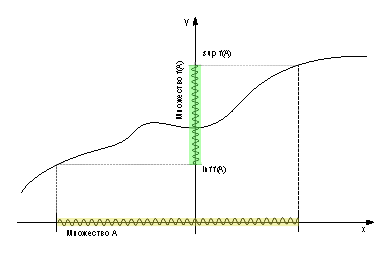
\includegraphics[width=3in]{lec_07_fig_01}
\end{figure}

Точной нижней гранью $f(x)$ на множестве $\mathbb{A}$ называется
\[\inf\limits_{x \in \mathbb{A}}f(x) = \inf f(\mathbb{A})\]

Точной верхней гранью $f(x)$ на множестве $\mathbb{A}$ называется
\[\sup\limits_{x\in \mathbb{A}} f(x) = \sup f(\mathbb{A})\]

\subsubsection{Возрастание и убывание функции на множестве}

Пусть $f: \mathbb{R} \mapsto \mathbb{R}$ и $\mathbb{A} \subseteq D(f)$, тогда
\begin{itemize}
  \item {
    $f(x)$ возрастает, если $\forall \underset{s < t}{s, t} \in \mathbb{A} \Rightarrow f(s) < f(t)$
  }
  \item {
    $f(x)$ не убывает, если $\forall \underset{s < t}{s, t} \in \mathbb{A} \Rightarrow f(s) \leq f(t)$
  }
  \item {
    $f(x)$ убывает, если $\forall \underset{s < t}{s, t} \in \mathbb{A} \Rightarrow f(s) > f(t)$
  }
  \item {
    $f(x)$ не возрастает, если $\forall \underset{s < t}{s, t} \in \mathbb{A} \Rightarrow f(s) \geq f(t)$
  }
\end{itemize}

\paragraph{Интересная взаимосвязь} Если $f$ возрастает, то верно и то, что она не убывает, однако
это не работает в обратную сторону

\end{document}
